\begin{figure}[!htb]
<<<<<<< HEAD
     {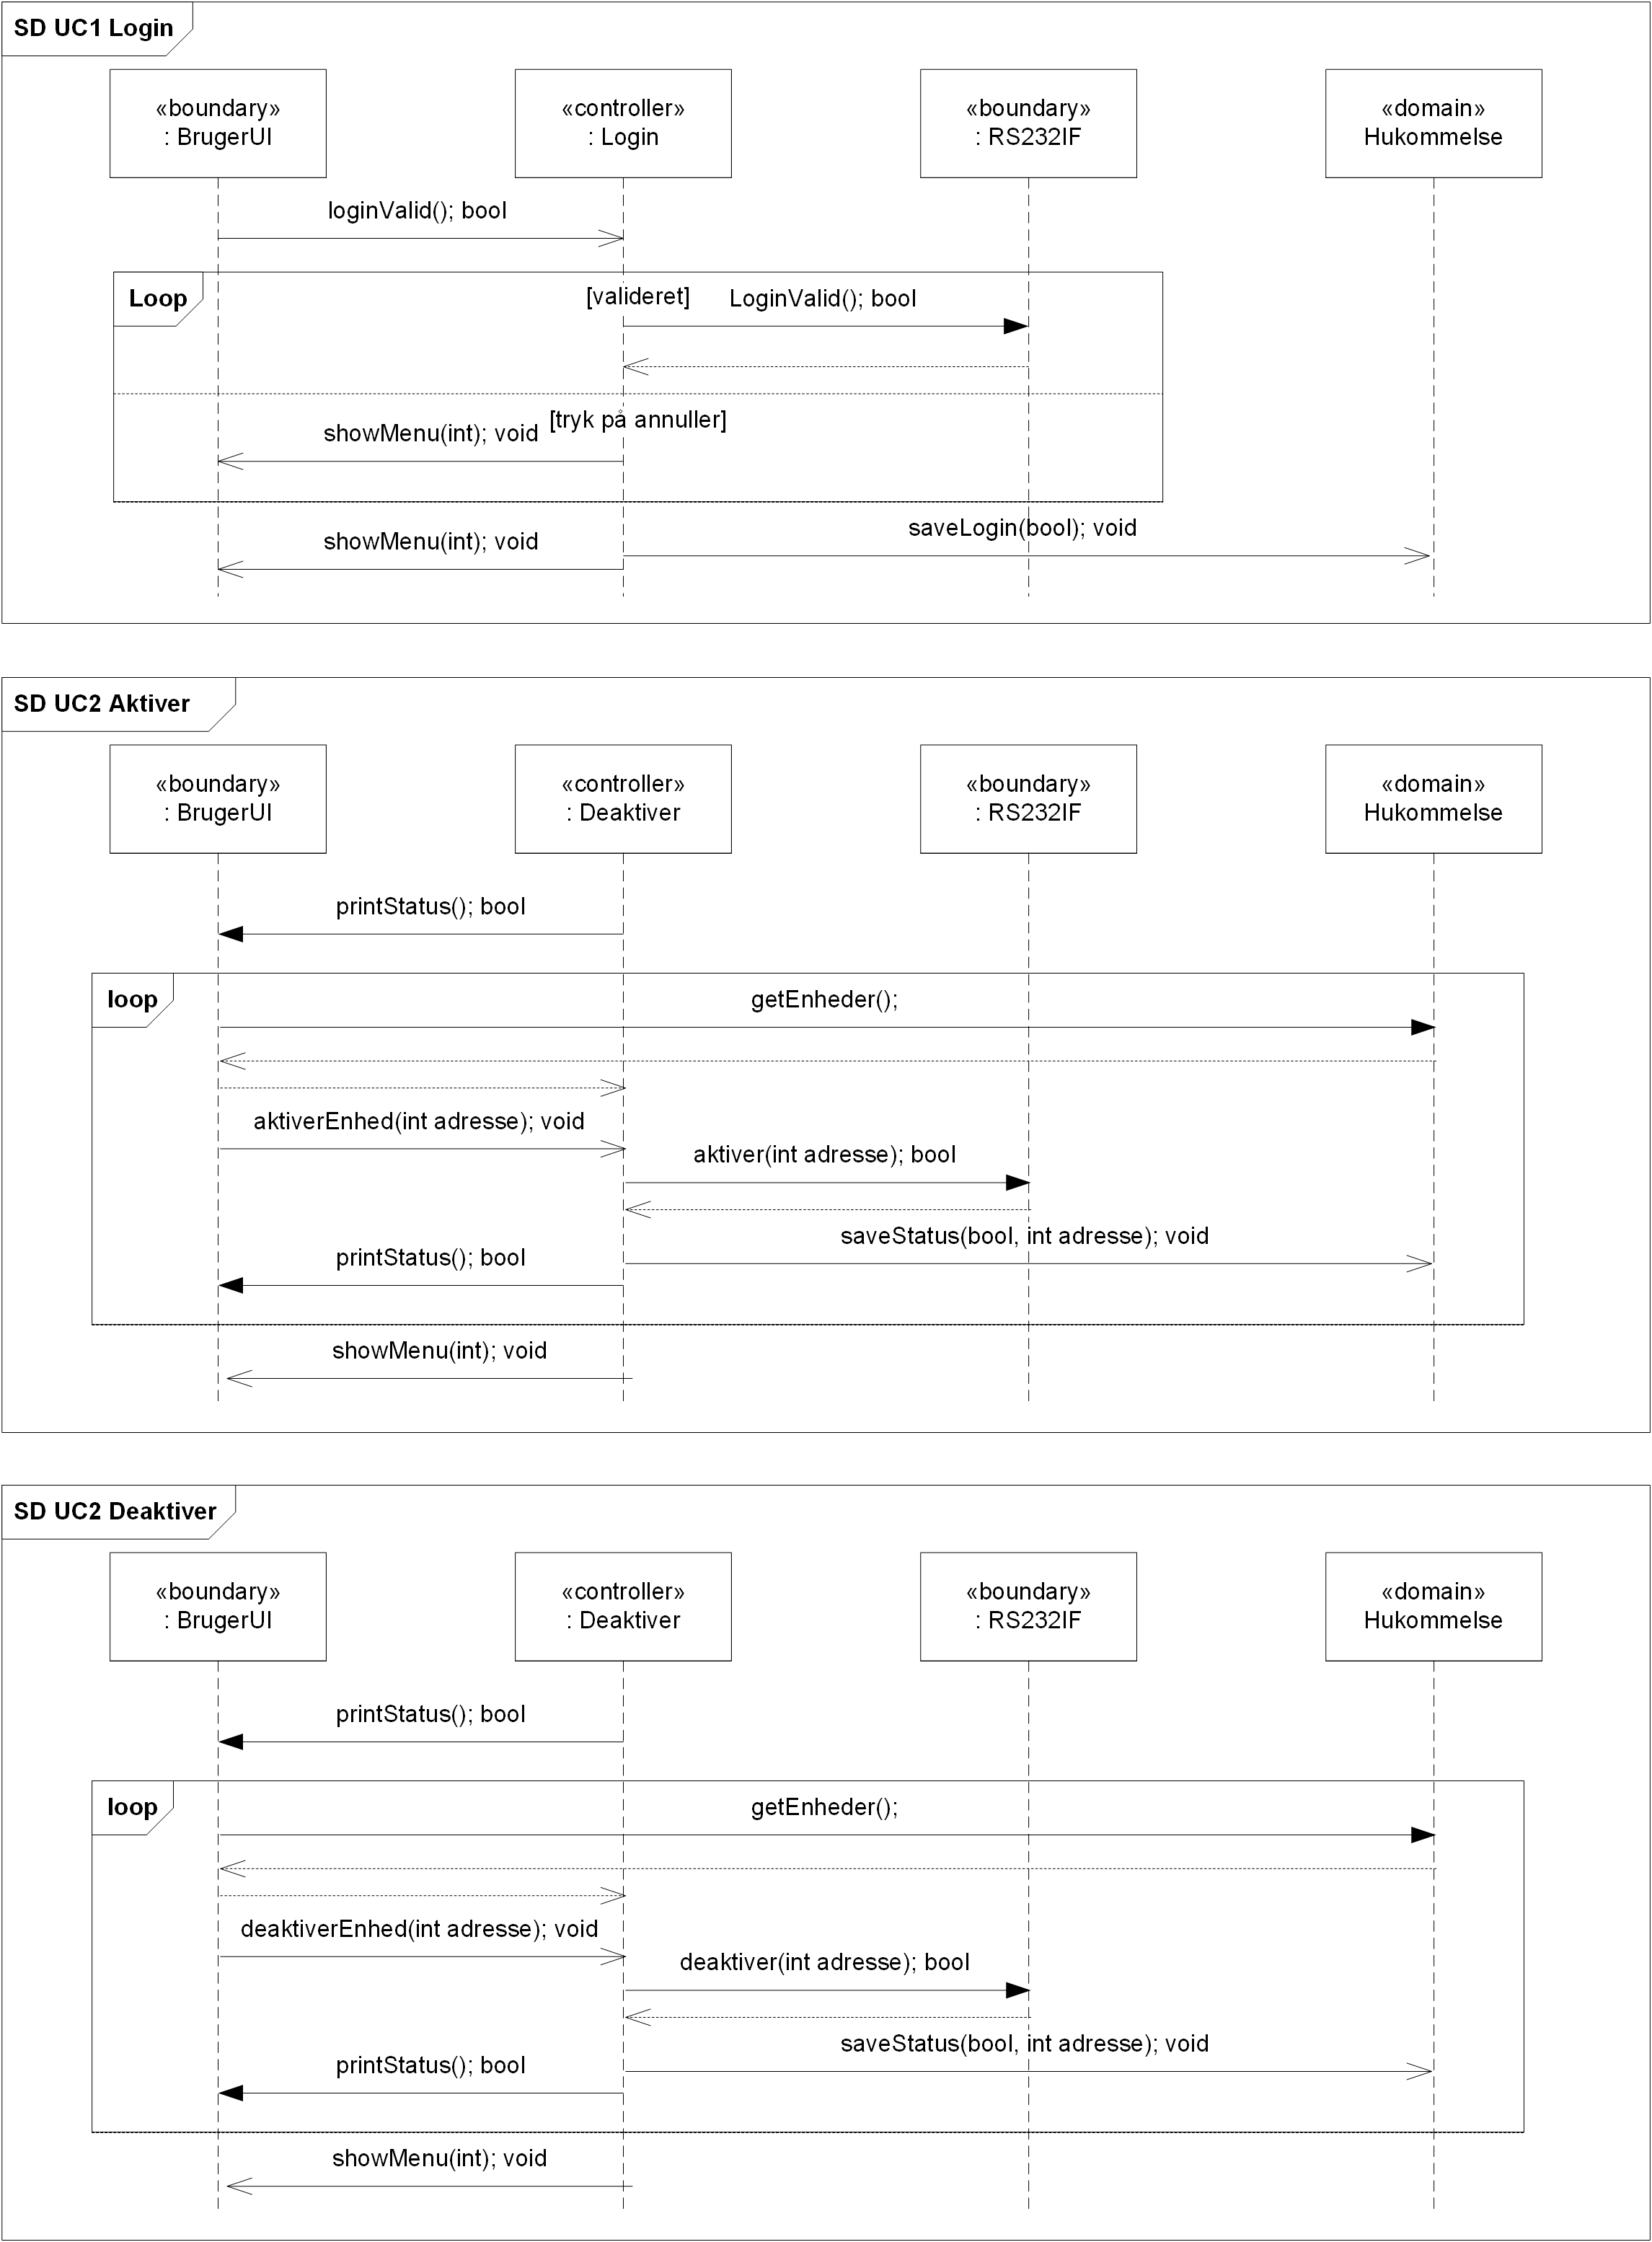
\includegraphics[width=\textwidth]{billeder/uml/PC_SD1}}
=======
     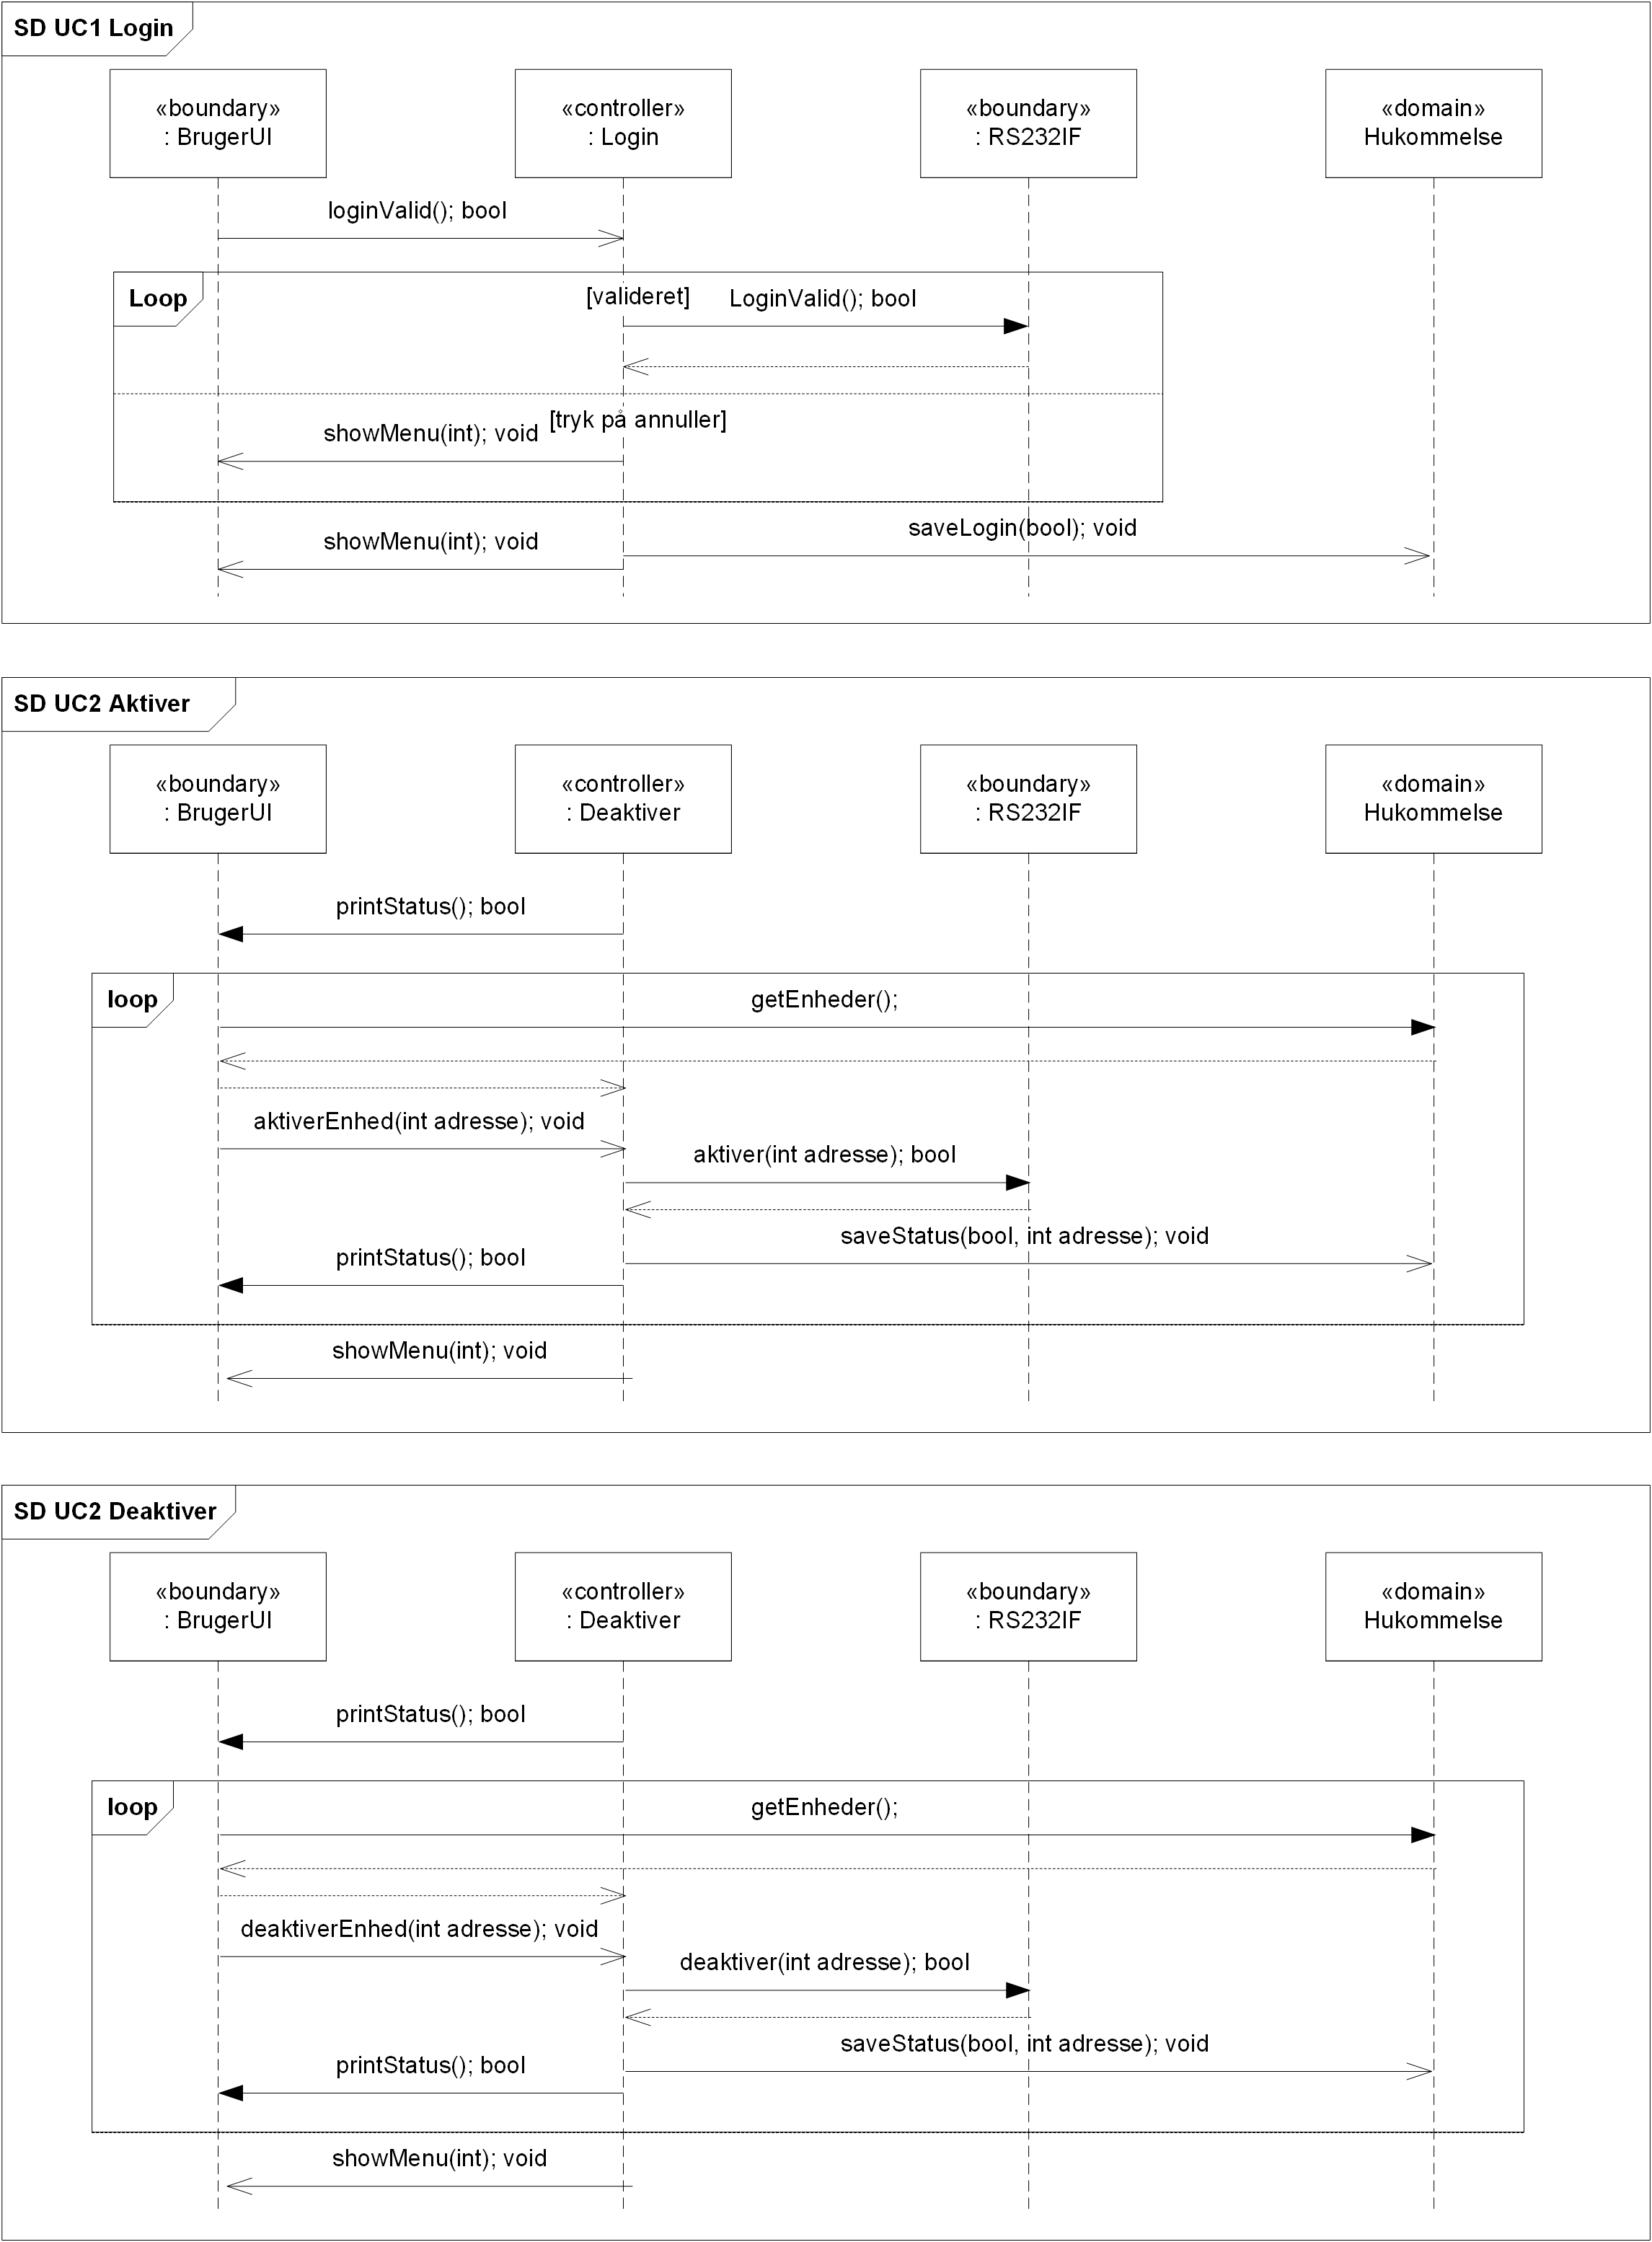
\includegraphics{billeder/uml/PC_SD1}
>>>>>>> FETCH_HEAD
     \caption{Use-case 1-3 sekvensdiagram for PC}
     \label{fig:PC_SD1}
\end{figure}

\begin{figure}[!htb]
<<<<<<< HEAD
     {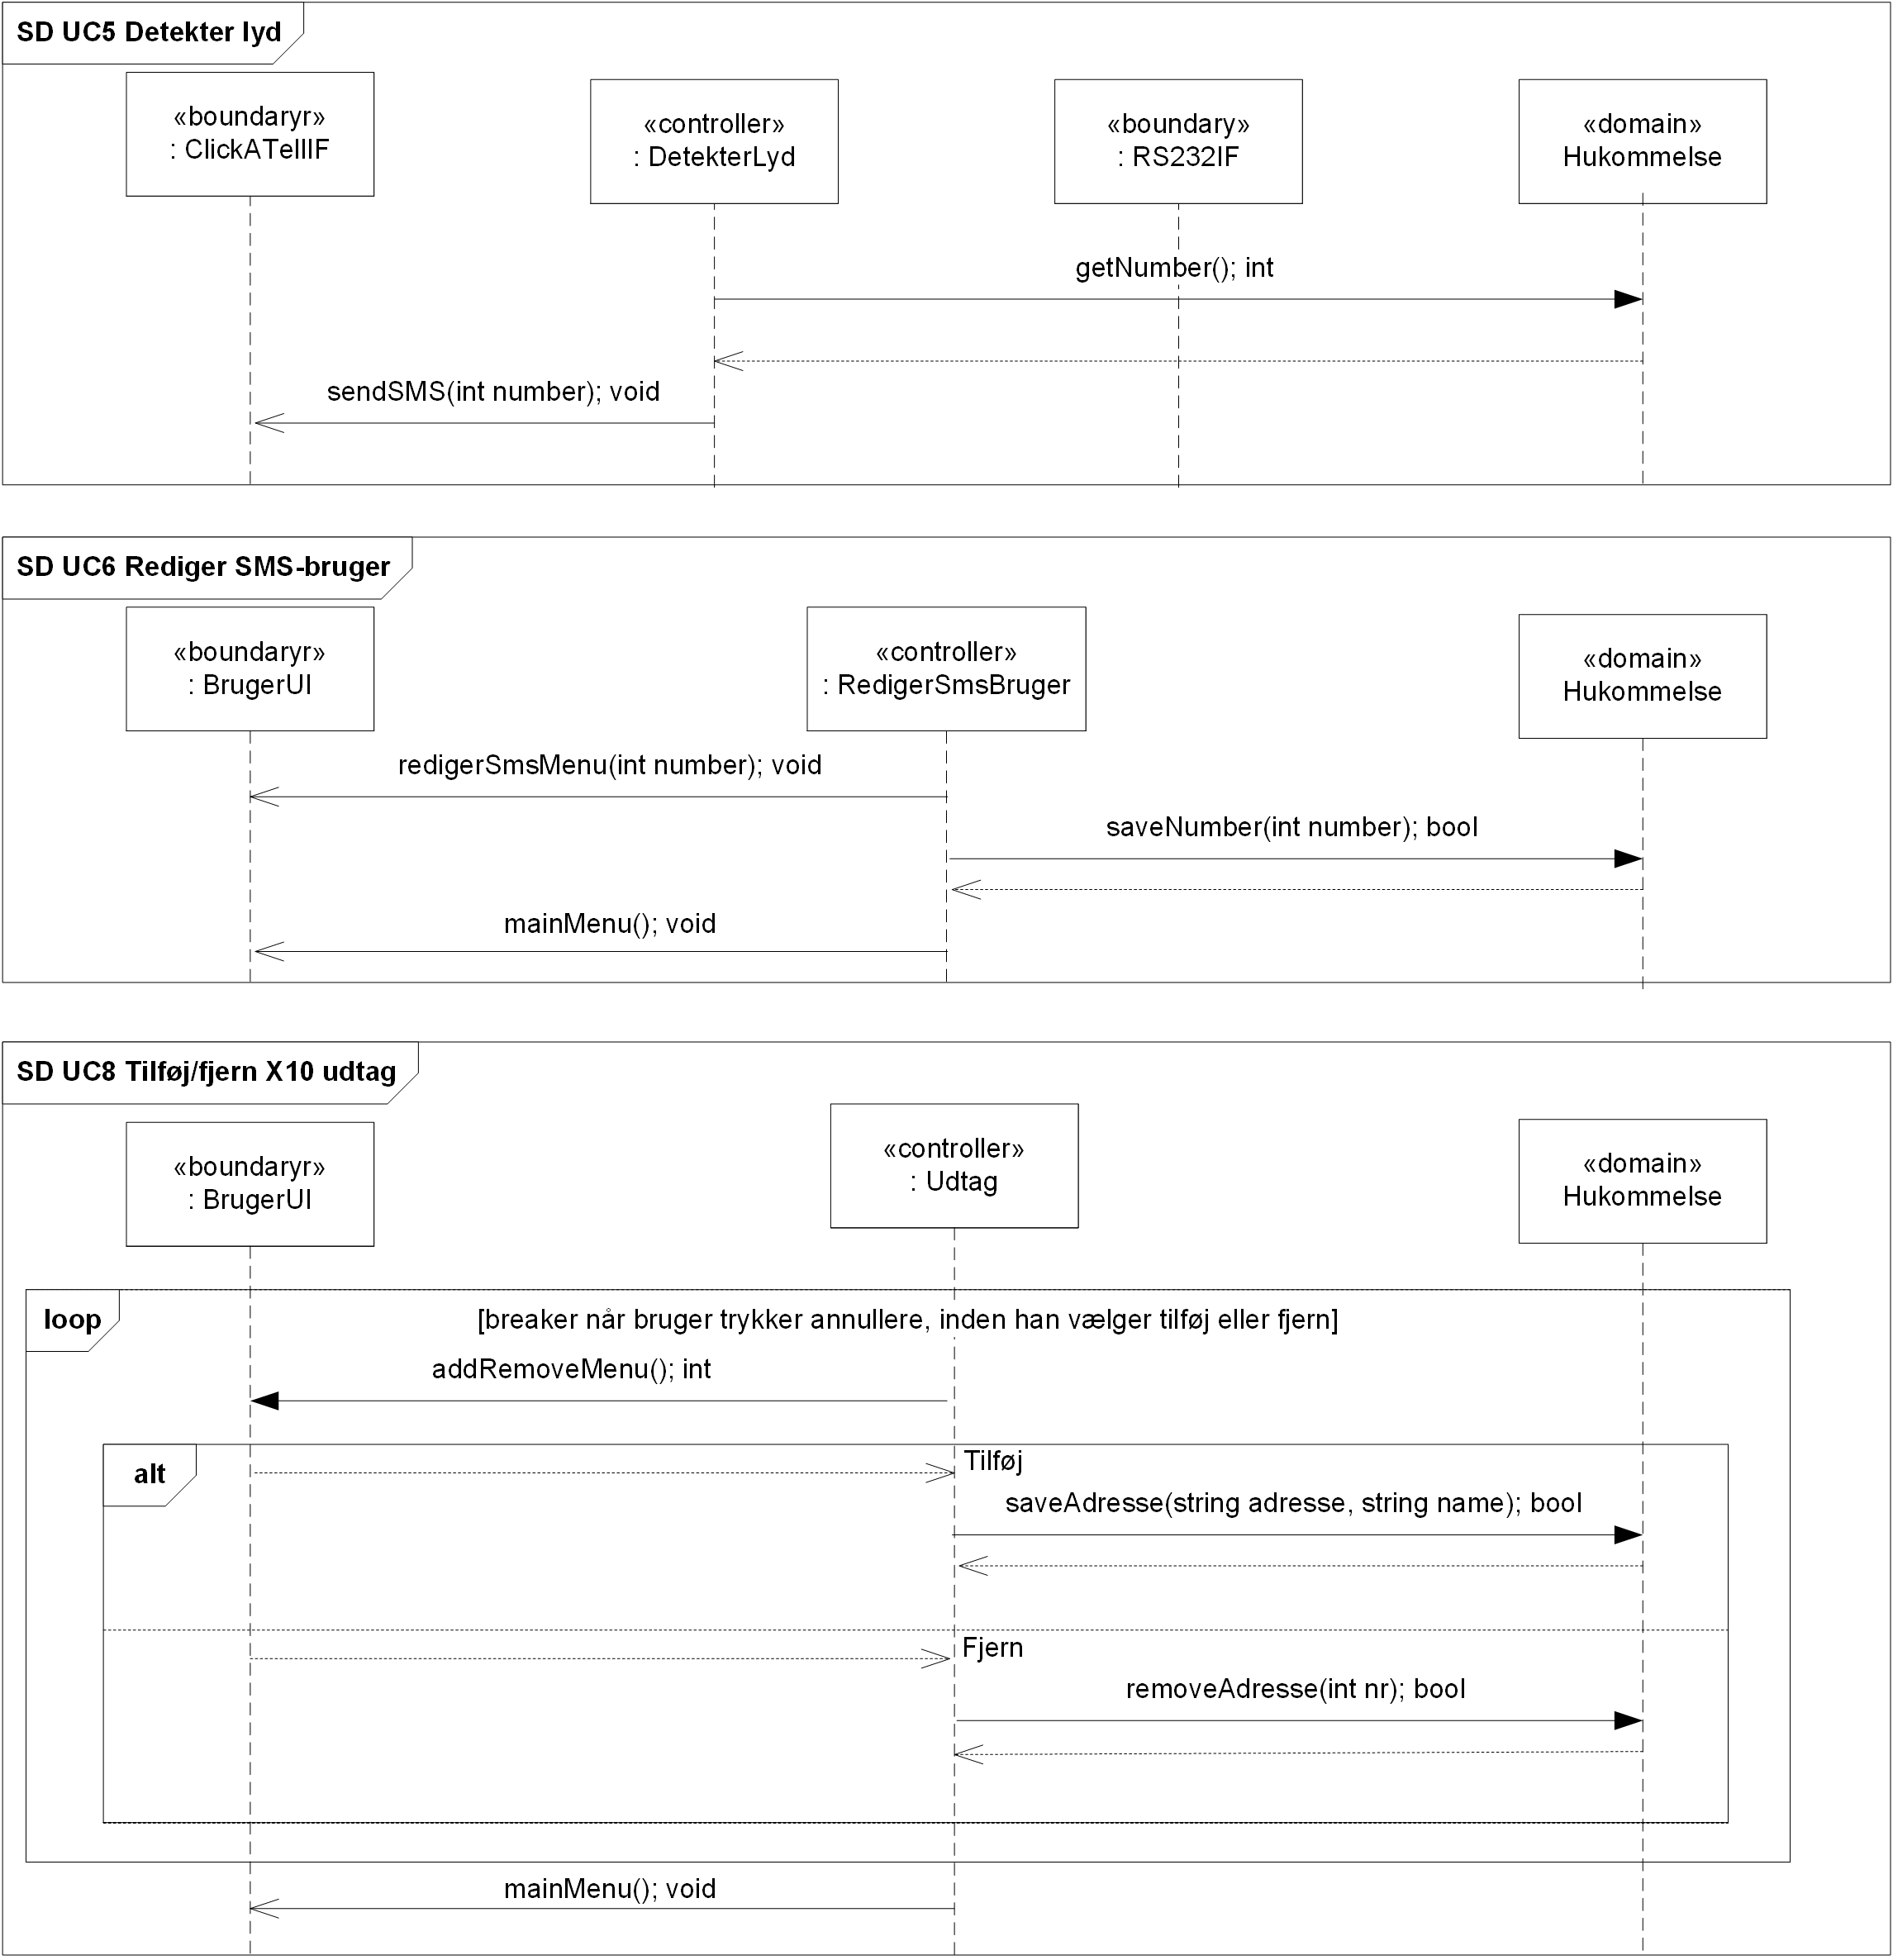
\includegraphics[width=\textwidth]{billeder/uml/PC_SD2}}
=======
     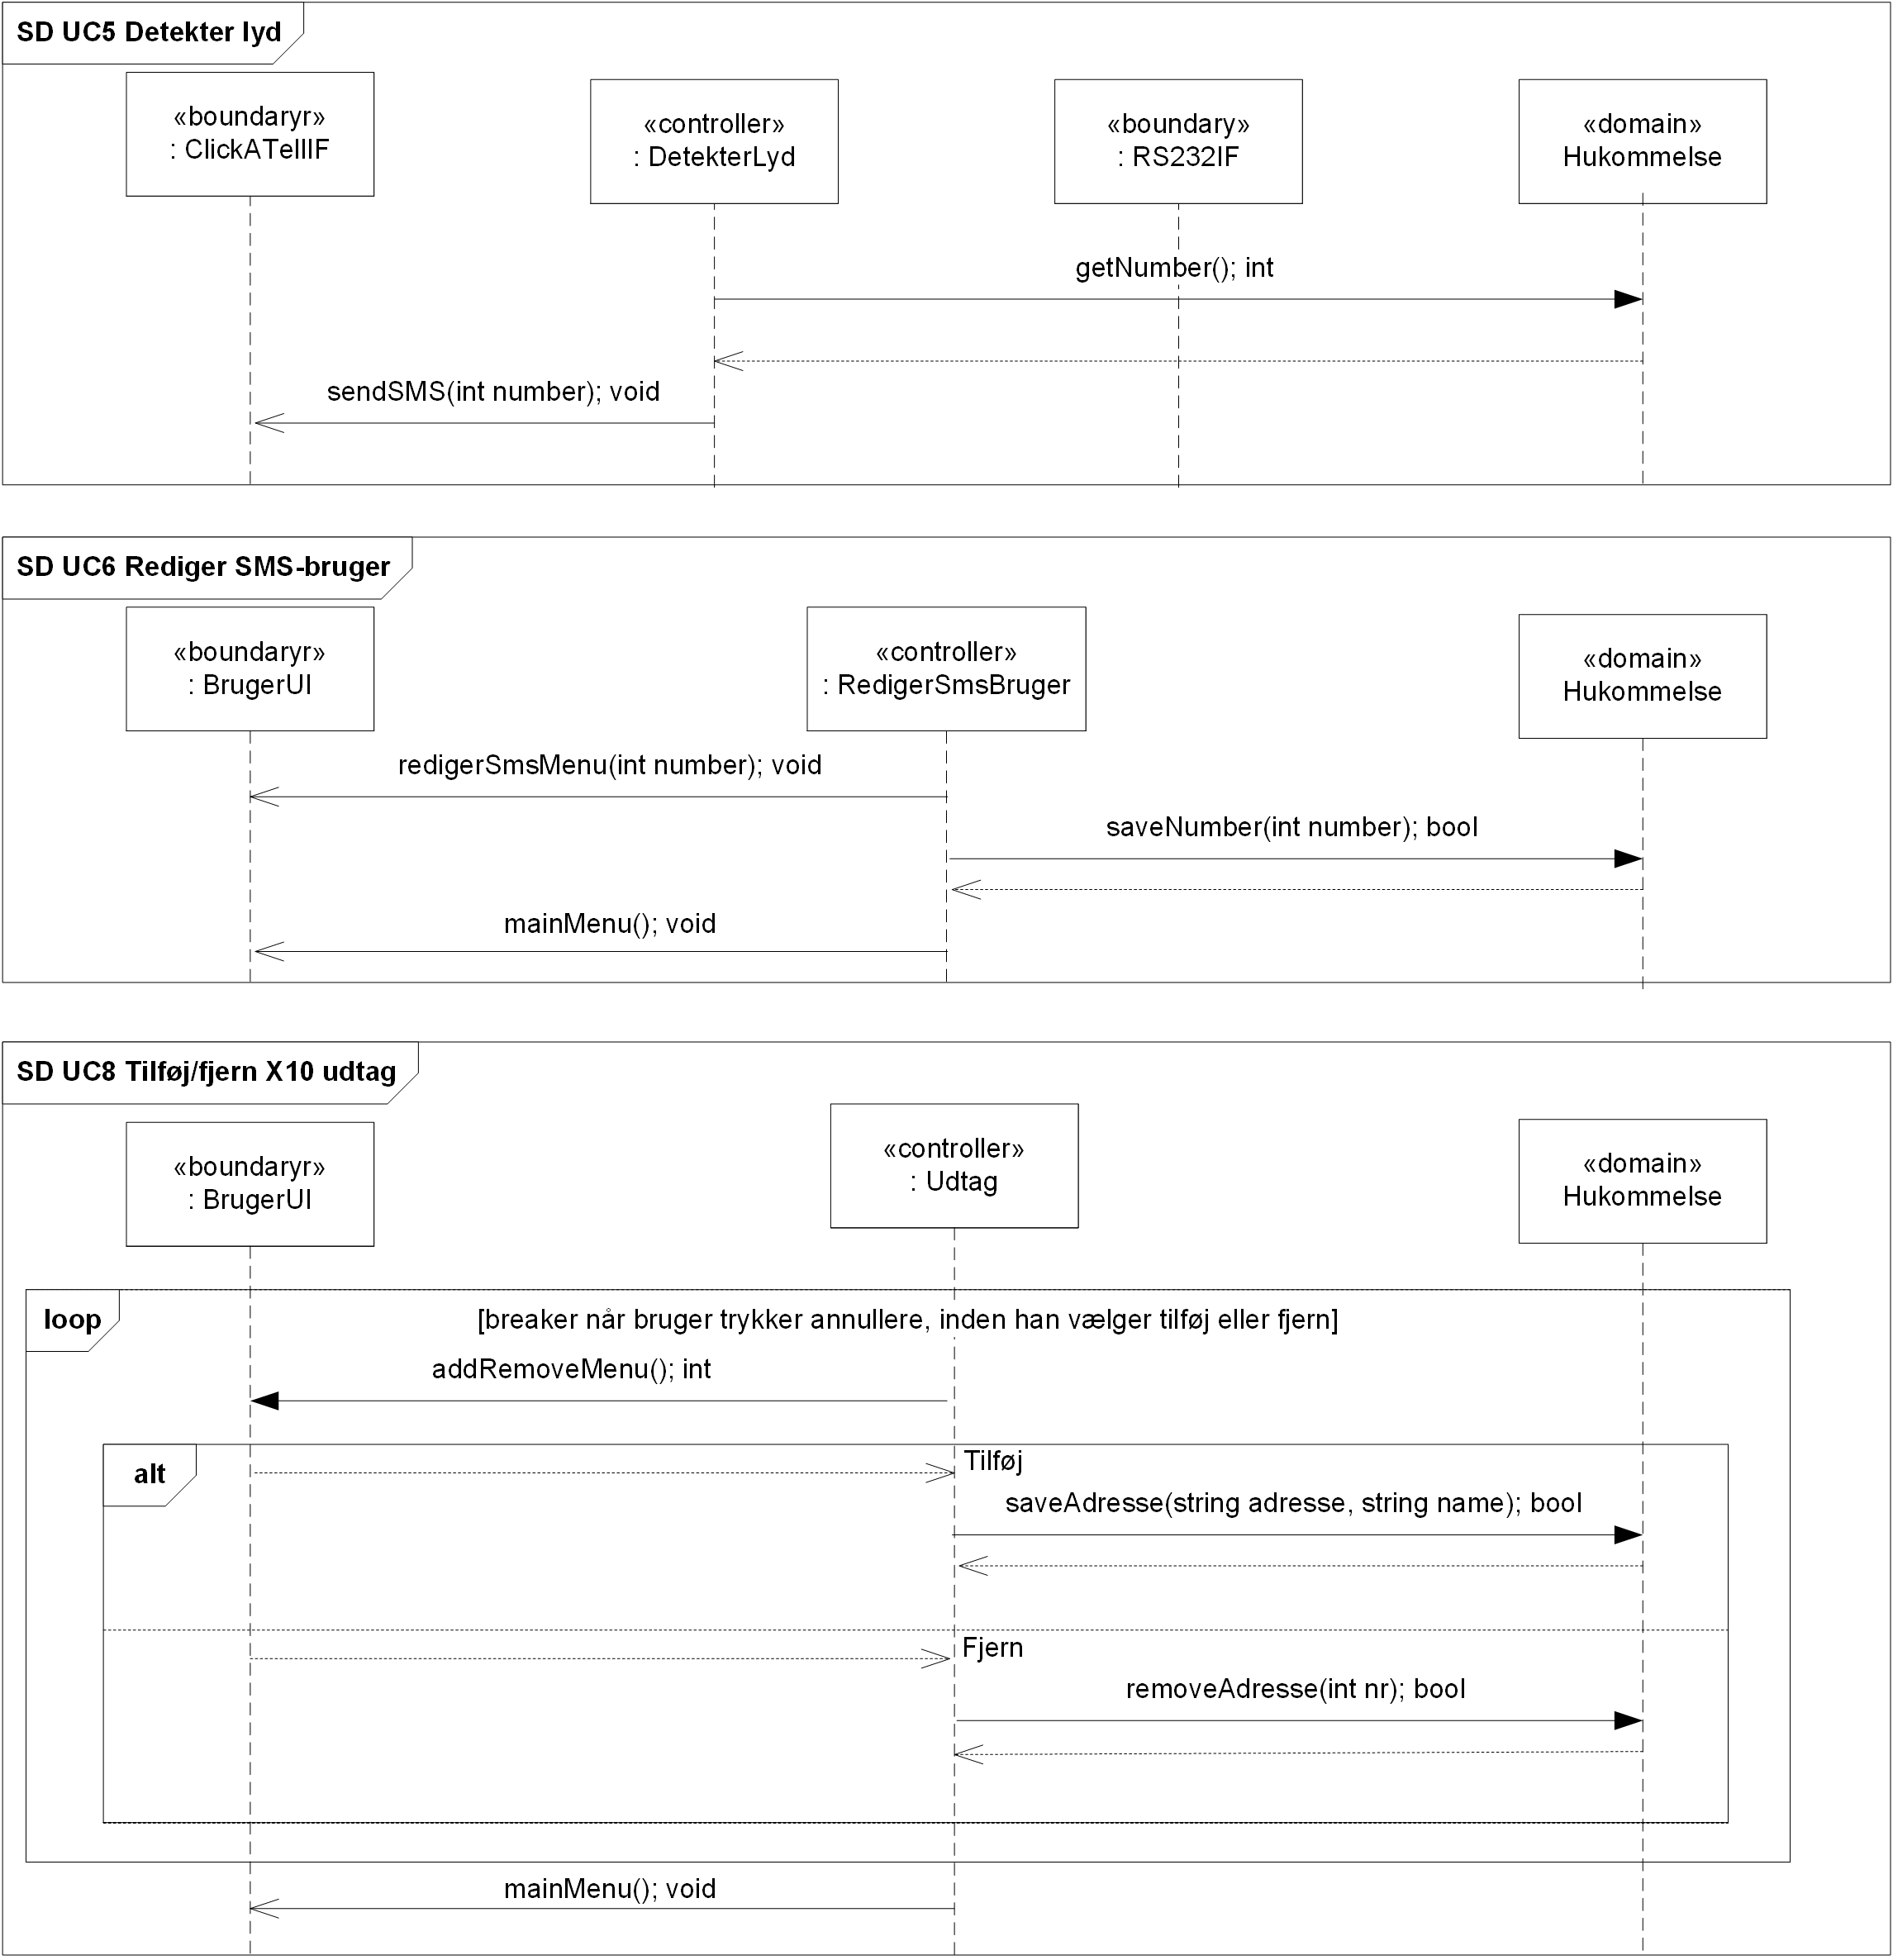
\includegraphics{billeder/uml/PC_SD2}
>>>>>>> FETCH_HEAD
     \caption{Use-case 5-8 sekvensdiagram for PC}
     \label{fig:PC_SD2}
\end{figure}

\begin{figure}[!htb]
<<<<<<< HEAD
     {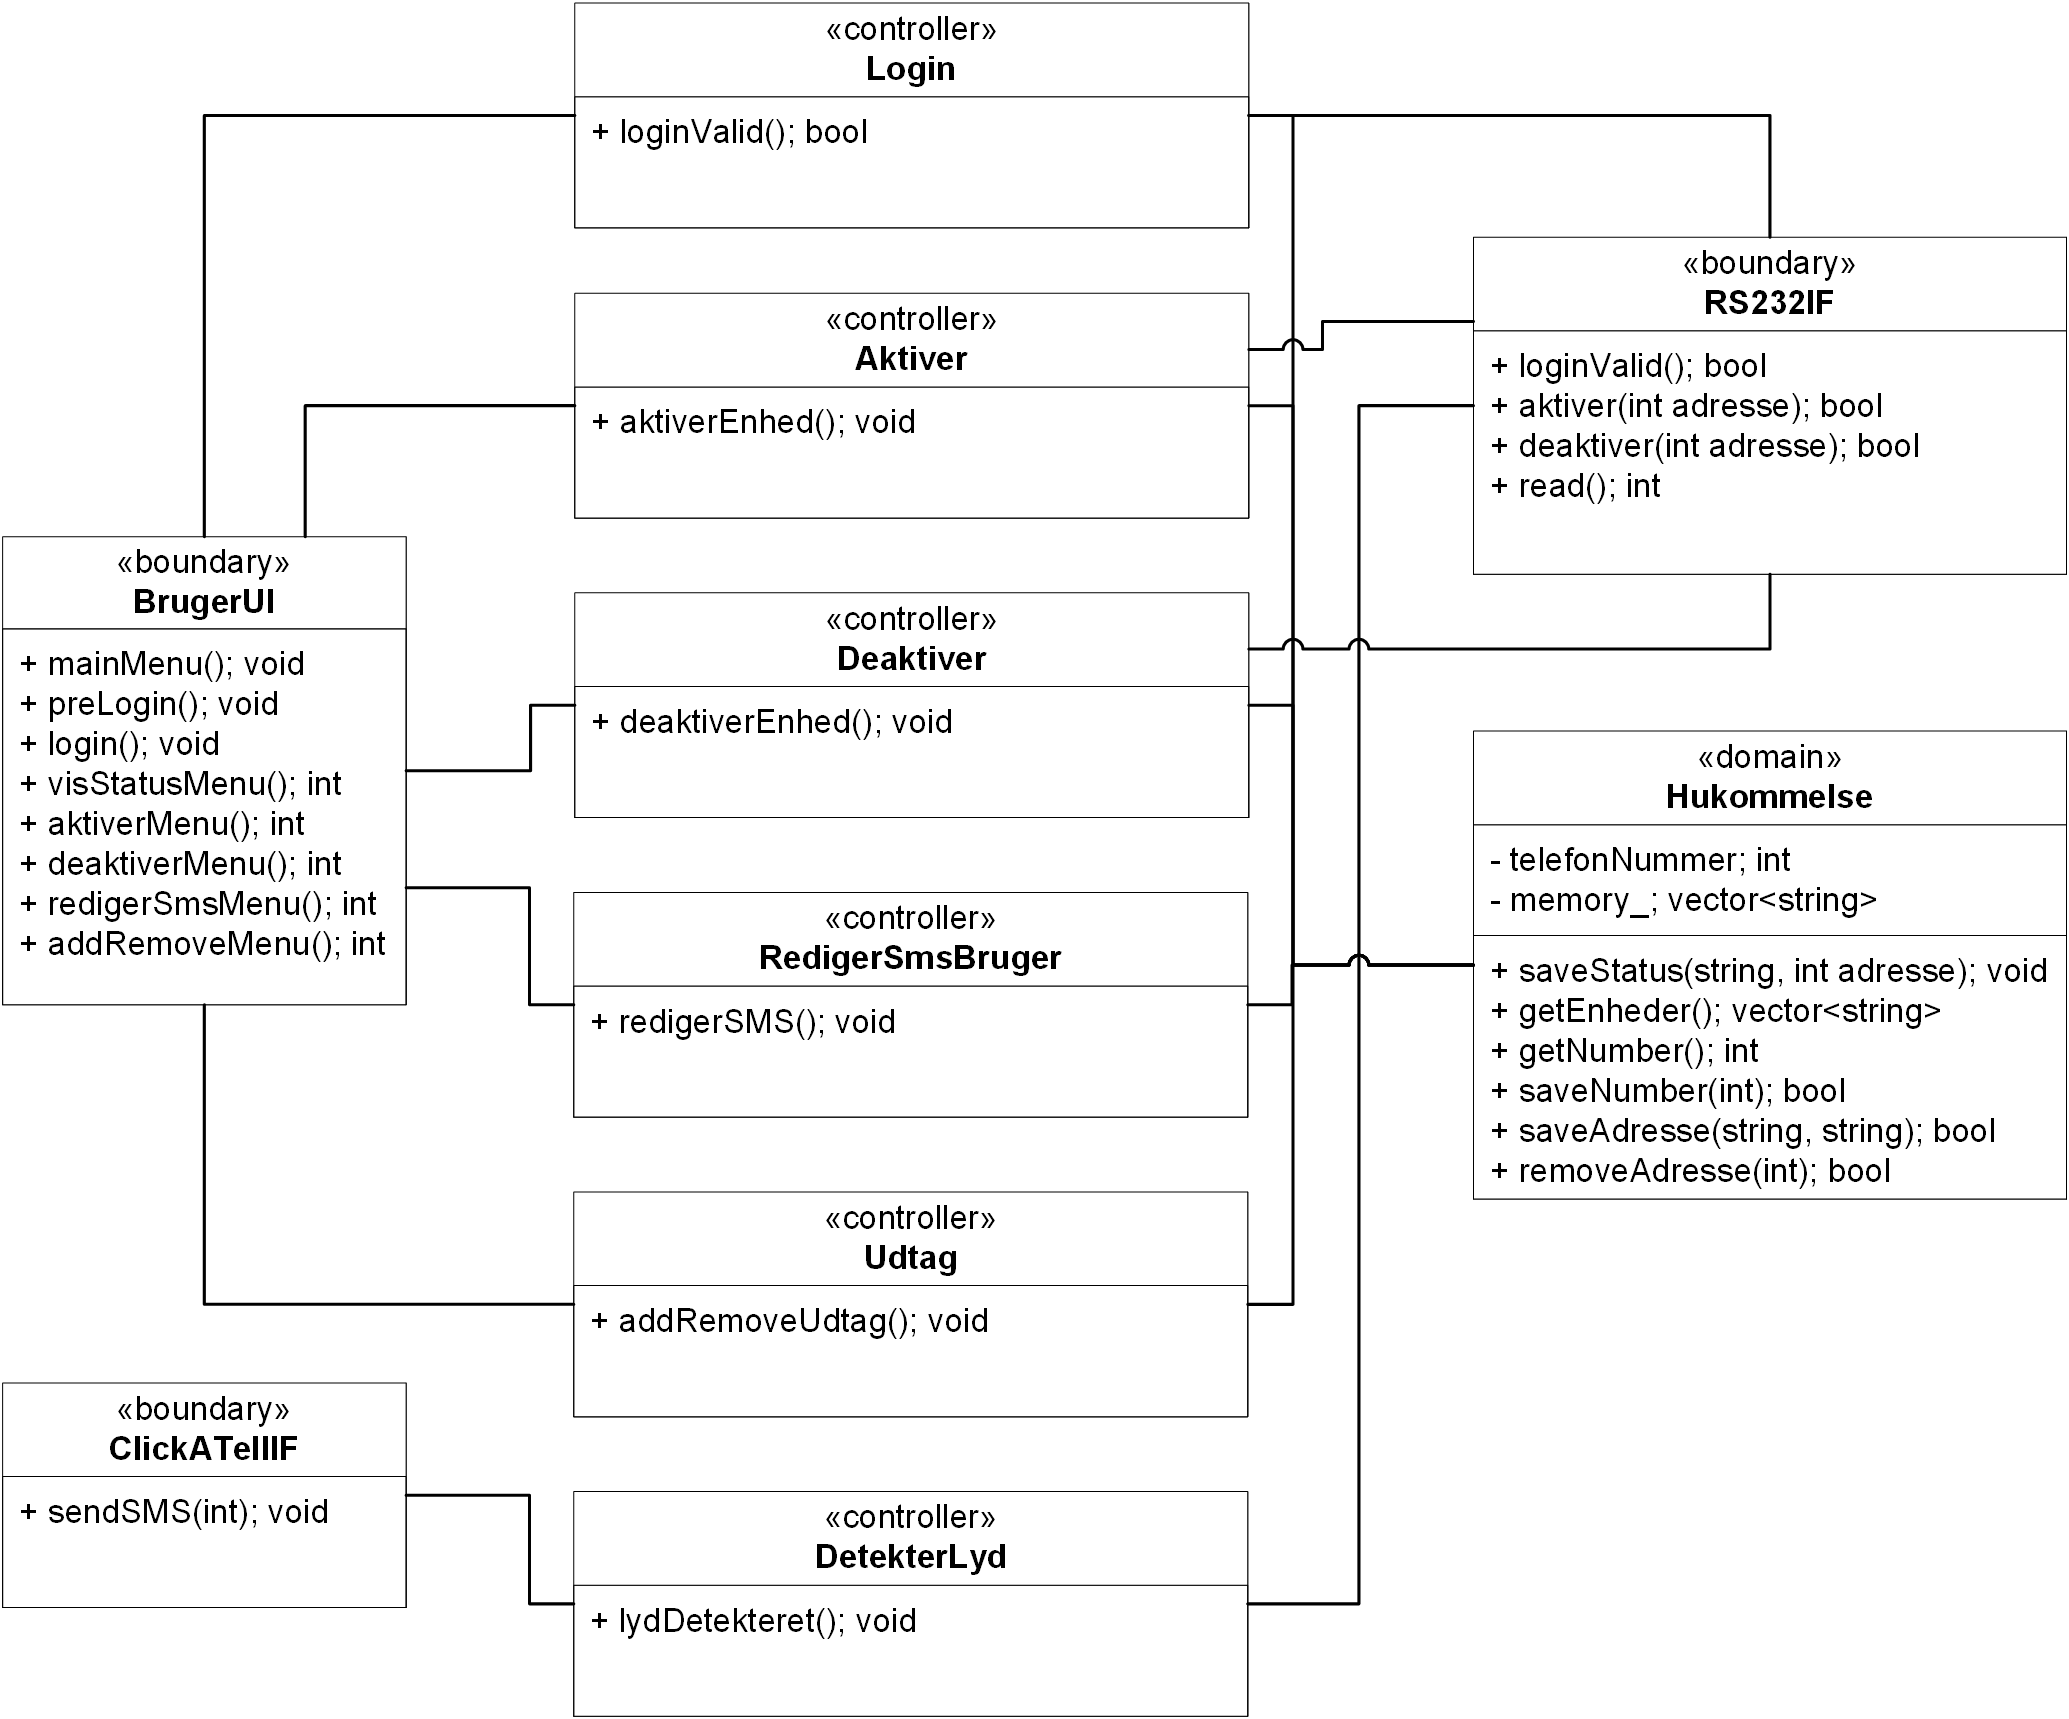
\includegraphics[width=\textwidth]{billeder/uml/PC_Class}}
=======
     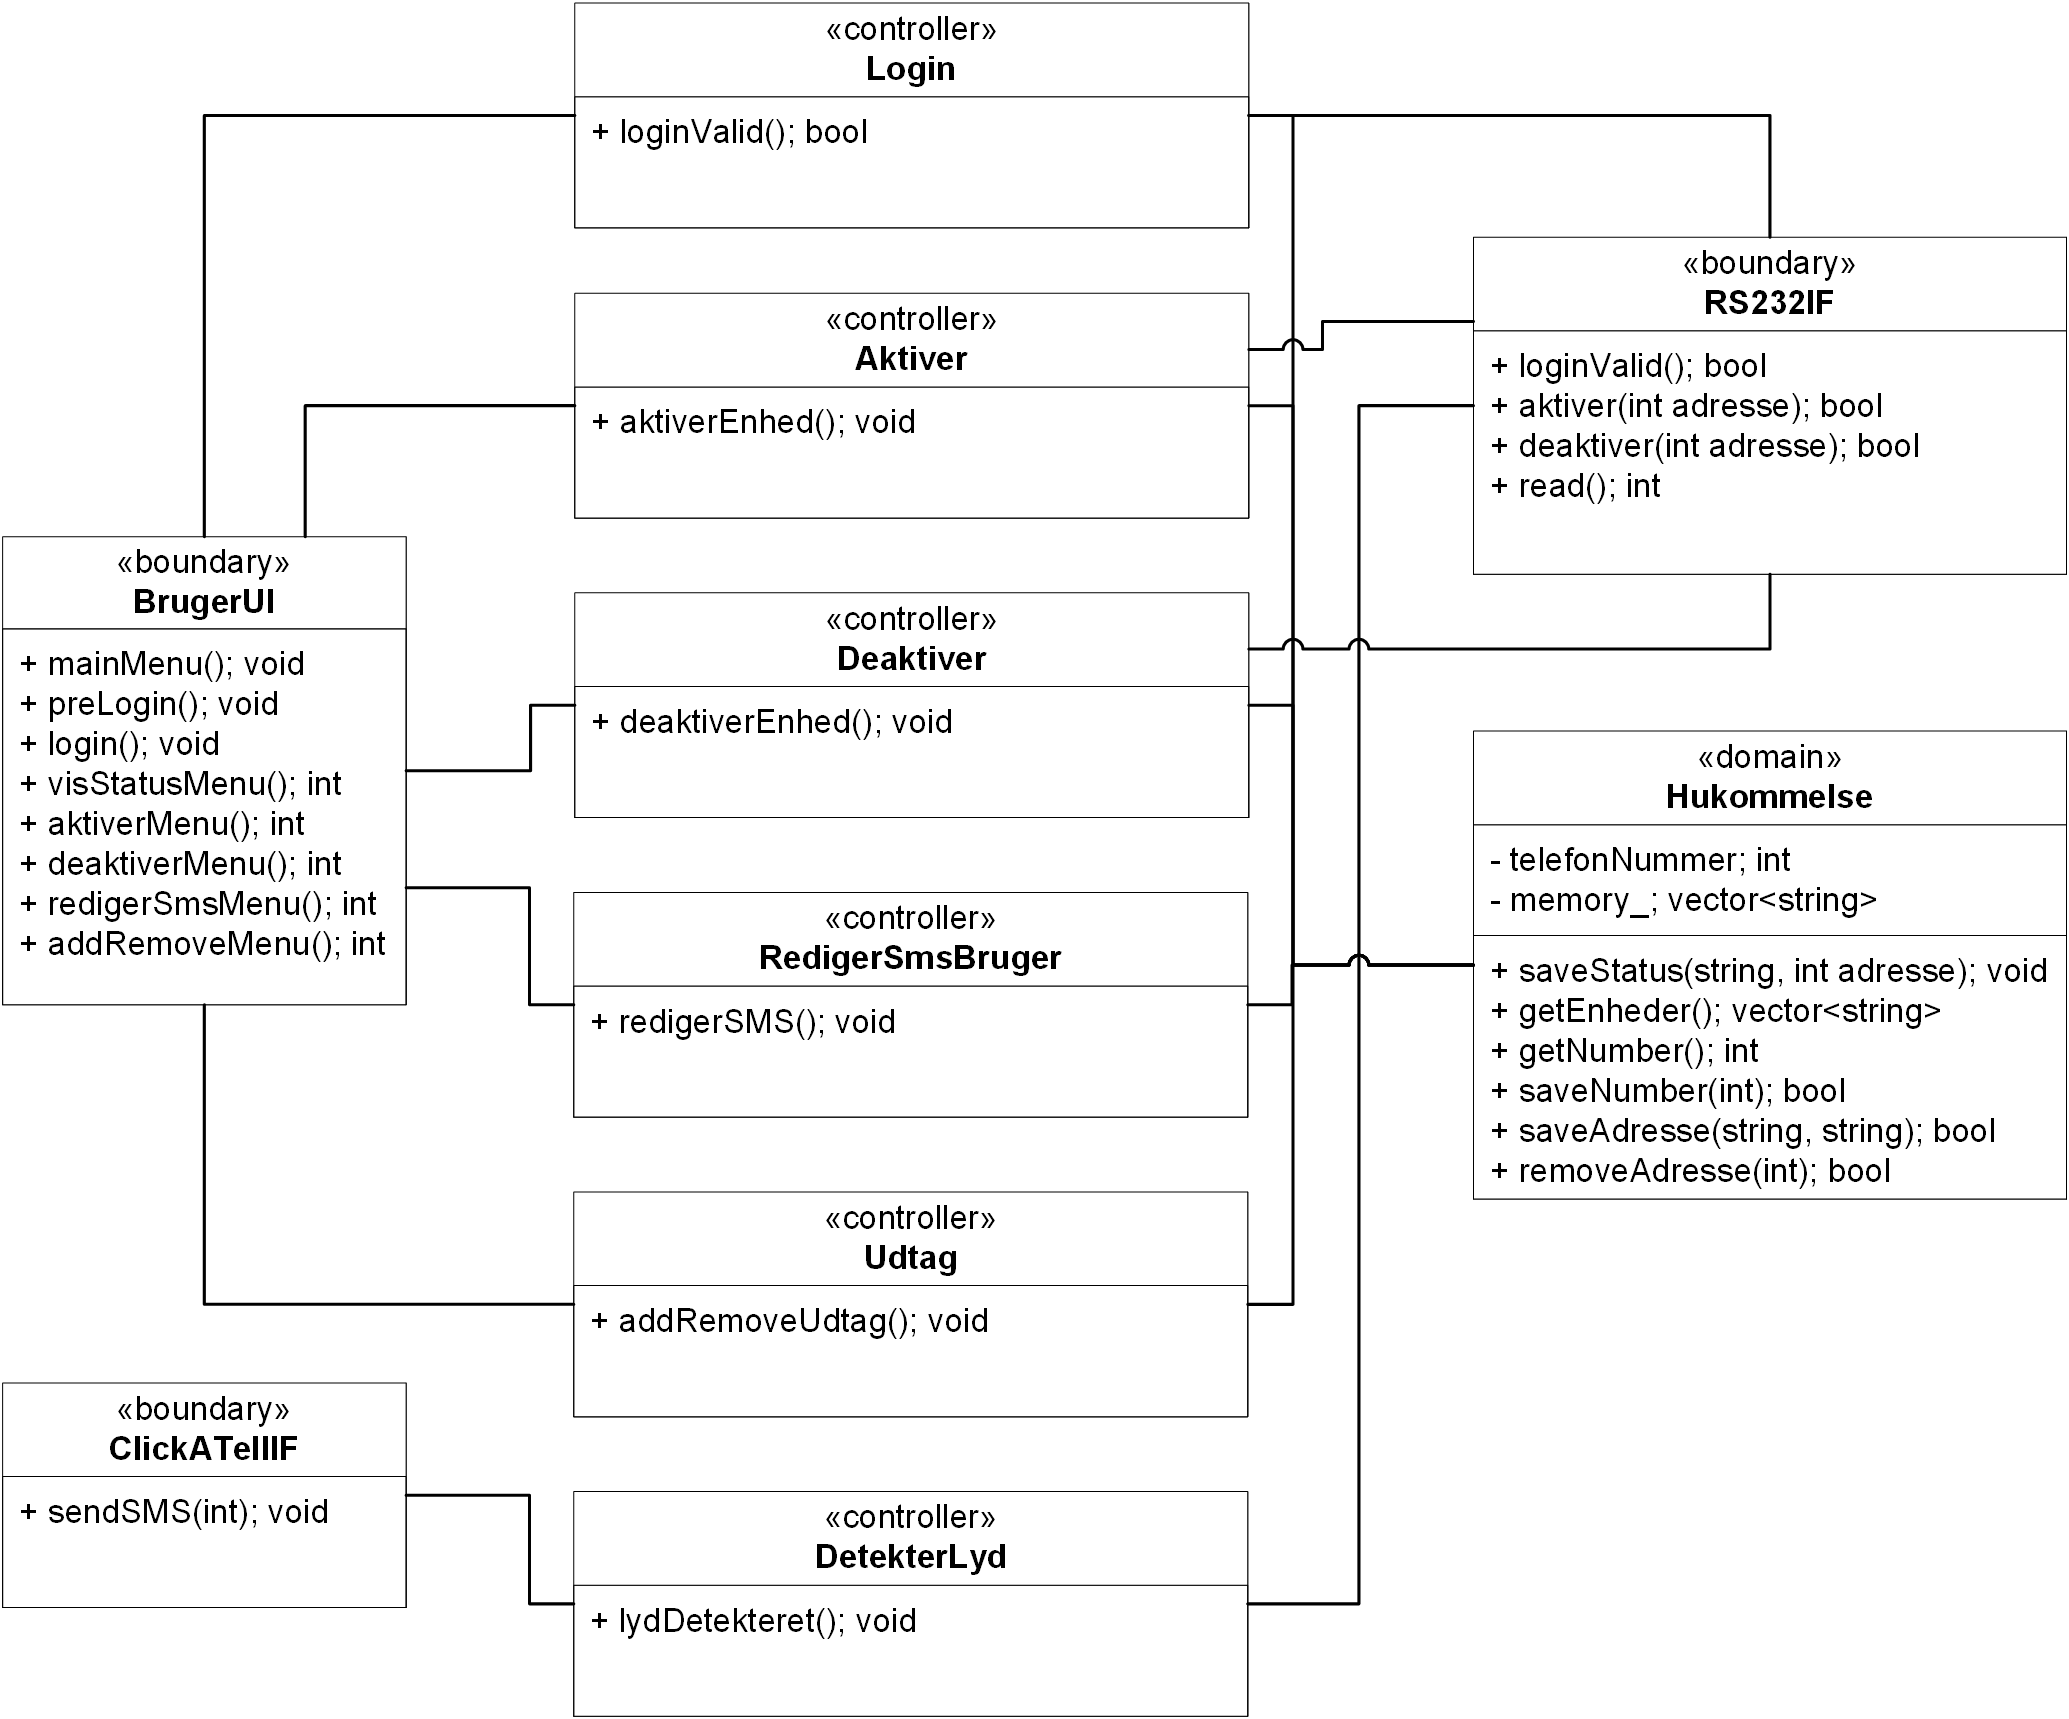
\includegraphics{billeder/uml/PC_Class}
>>>>>>> FETCH_HEAD
     \caption{Klassediagram for PC}
     \label{fig:PC_Class}
\end{figure}
%
%\begin{figure}[!htb]
%     \xput[0.471]{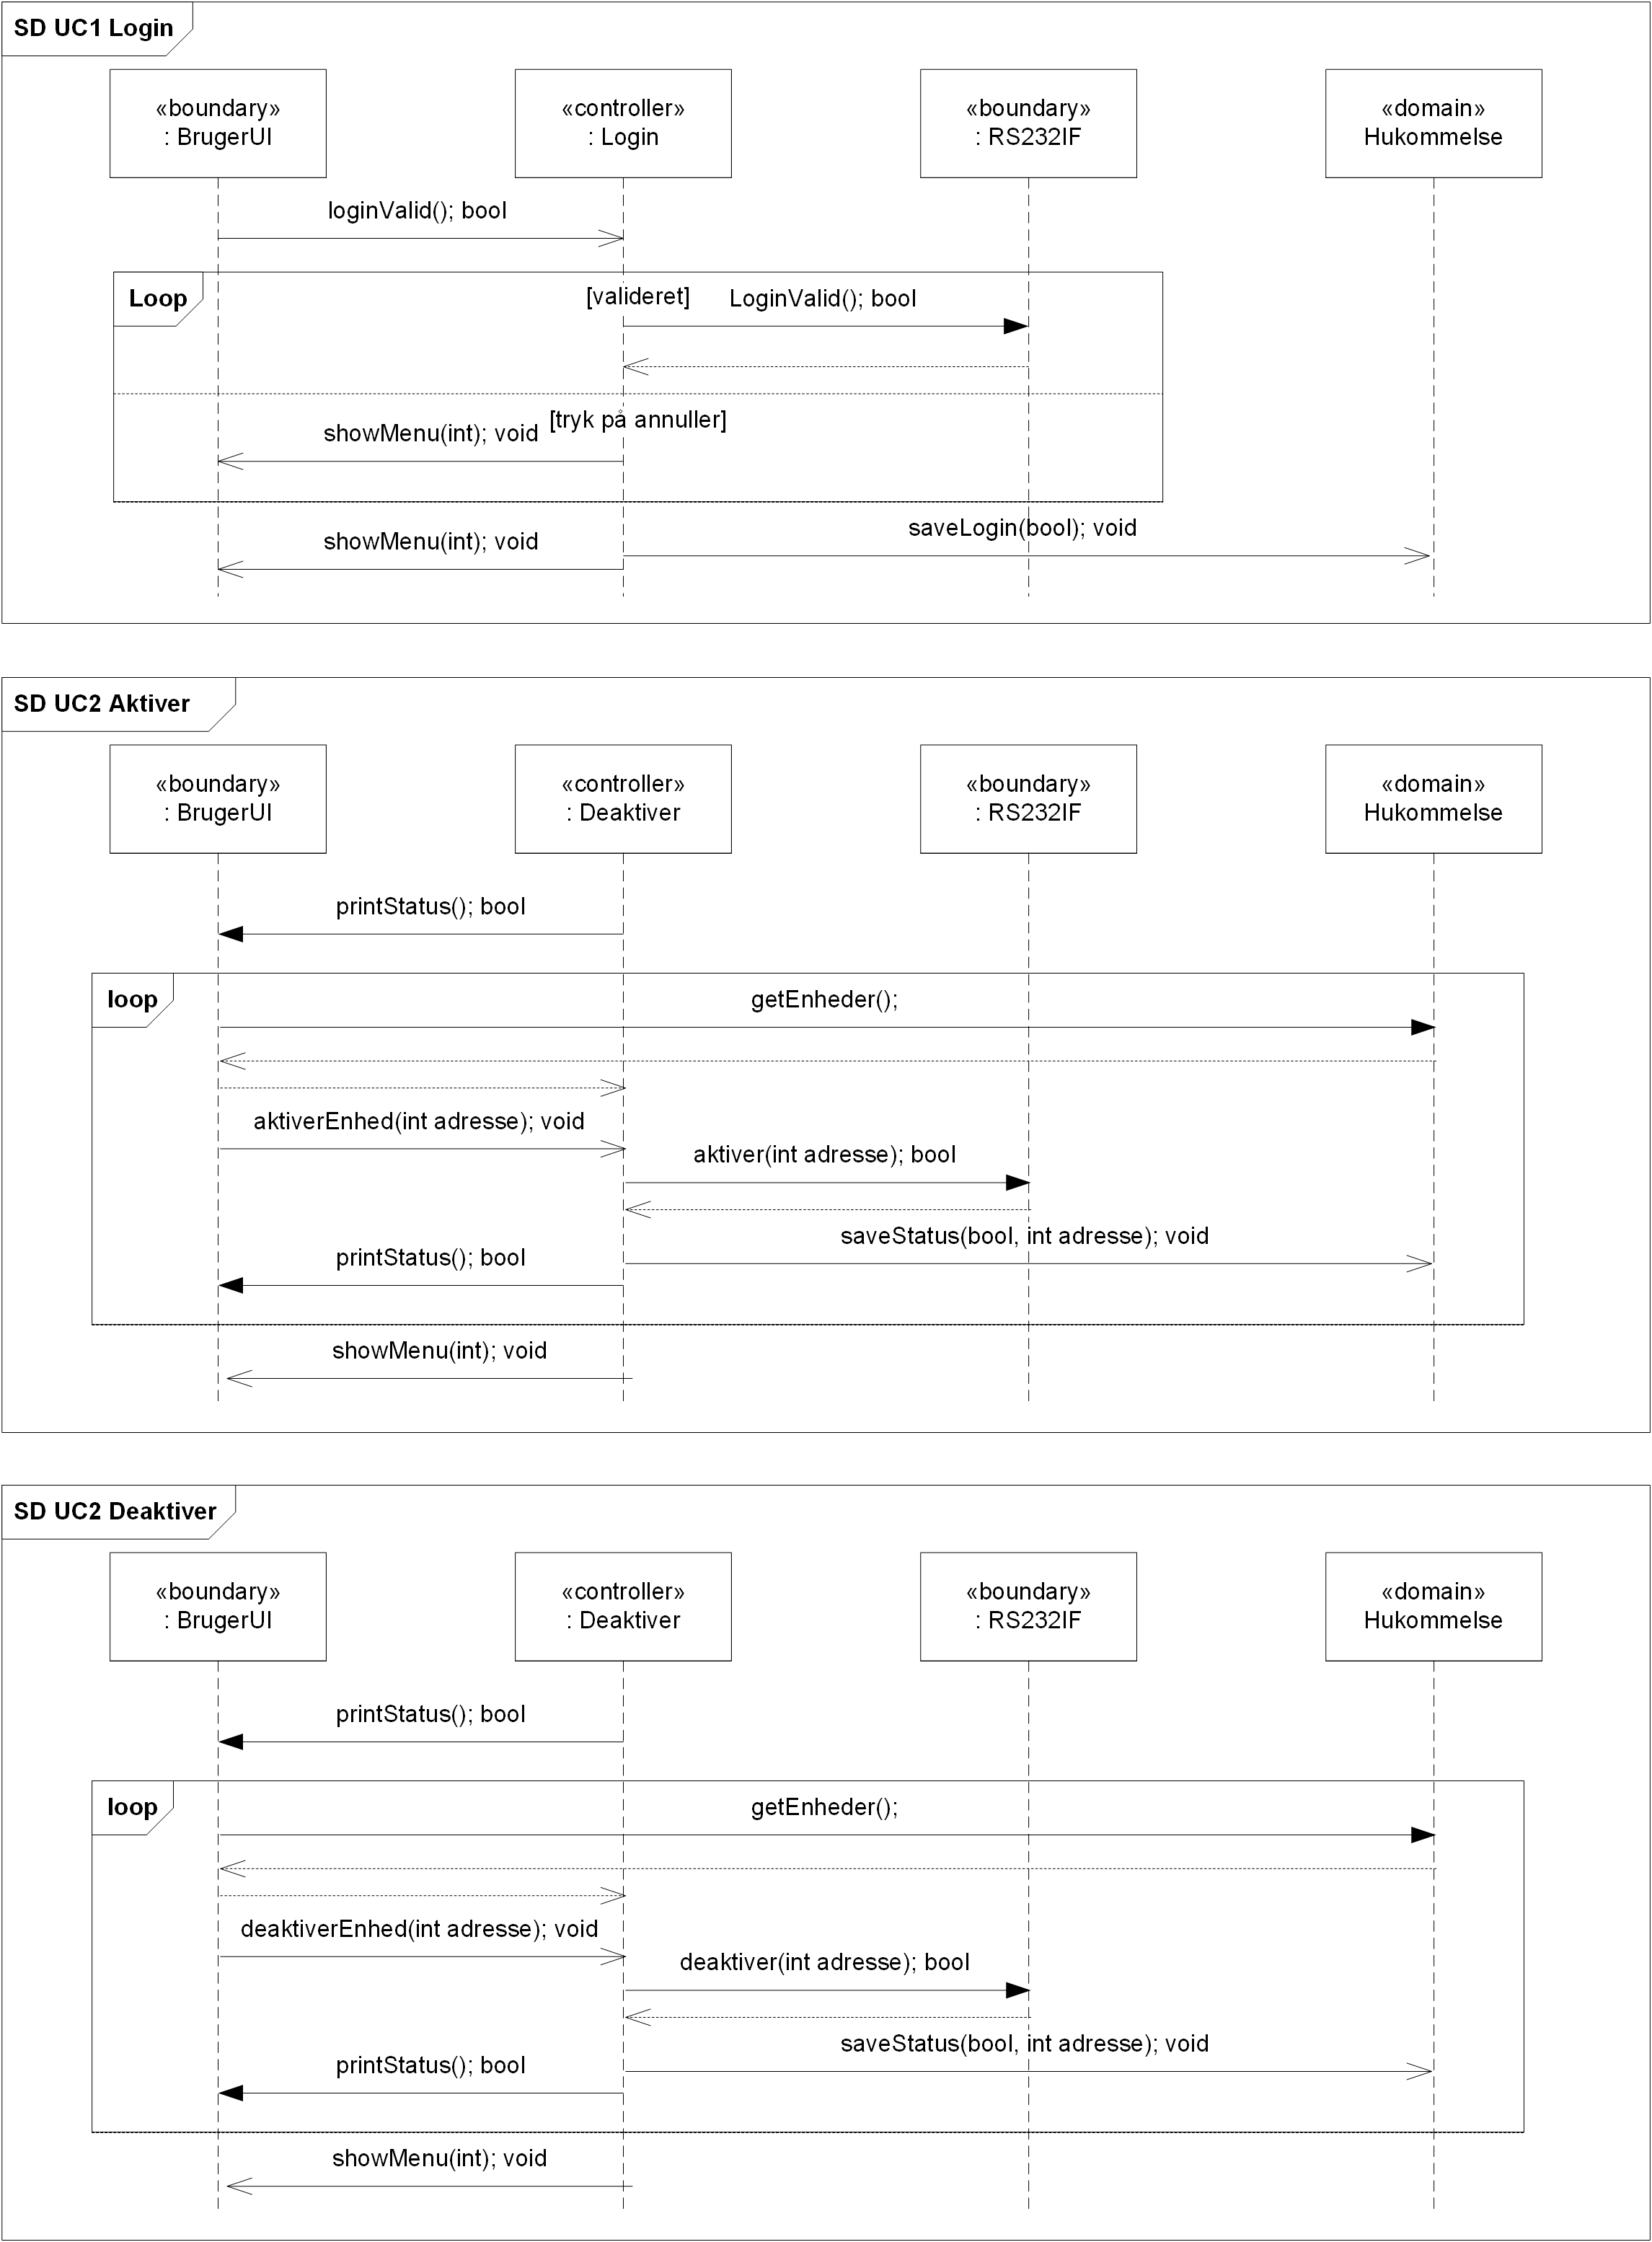
\includegraphics[width=1.32\linewidth]{billeder/uml/PC_SD1}}
%     \caption{Use-case 1-3 sekvensdiagram for PC}
%     \label{fig:PC_SD1}
%\end{figure}
